\section{Grundlagen}
 
\subsection{Objekt-Relationale Unverträglichkeit}

In einem Softwareparadigma manifestiert sich ein bestimmtes Konzept in der Modellierung der Welt. Durch diese konzeptionelle Betrachtungsweise beeinflusst ein Paradigma den Erstellungsprozess sowie die Ergebnisse des Softwaredesigns und zwingt diesem seine Grenzen auf. Probleme bei der Kombination verschiedener Paradigmen werden dabei als Unverträglichkeit (impedance Missmatch) bezeichnet.
Objektorientierte Programmierung  und eine relationale Abfrage von Datensätzen sind weit verbreitete Paradigmen in der Softwareentwicklung. Damit ist die objekt-relationale Unverträglichkeit (object-relational impedance mismatch) eine häufig auftretende Herausforderung. (vgl. \cite{ireland2009classification} S. 36-38)\\

\cite{ireland2009classification} nennt dabei unter anderem folgende Betrachtungsweisen als Ursachen für die objektrelationale Unverträglichkeit.

\begin{description}
 \item [Strukturelle Unterschiede]  
 Die objektorientierte Programmierung erlaubt das definieren, beliebig komplexer Strukturen aus Methoden und Klassen. Durch Vererbungsstrukturen ist es möglich, Objekte zu spezialisieren und Konzepte für die Erstellung der Klassen zu generalisieren. Spricht man von einer relationalen Algebra, diese wird durch Tupeln, Mengen und Wahrheitswerten definiert. Inhärent wiederholbare Strukturen oder Hierarchien können mit diesen Mitteln nicht umgesetzt werden.   
 
 \item [Datenkapselung] 
 In der objektorientierten Programmierung können die intrinsischen Attribute eines Objektes verborgen werden. Dieses Konzept sit als Kapselung bekannt und erlaubt es den Zugriff auf die gekapselten Strukturen einzuschränken. In einer relationalen Algebra ist eine derartige Abstraktion über die Daten nicht vorgesehen.
 
 
 \item [Objektidentität]  
 Durch die Instanziierung eines Objektes aus einer Klasse erhält dieses eine eindeutige Identität, somit unterscheiden sich zwei Objekte auch wenn diese träger eines identischen Datensatzes sind, durch ihre Repräsentation im Arbeitsspeicher. Relationen werden durch den Primärschlüssel, und damit über ihre Daten, definiert. Zwei eigenständige Relationen mit identischem Datensatz ist damit nicht möglich.
\end{description}


Als Hilfsmittel zur Überwindung der oben genannten Probleme werden Objekt-Realtionale Mapper (ORM bzw. O/R-Mapper) eingesetzt. Durch dieses Mapping wird eine Schnittstelle oder Abstraktionsebene zwischen Programmteilen aus den jeweiligen Sprachparadigmen definiert, um den impedance Mismatch möglichst transparent zu überwinden.



%% TODO: Vorstellung der in SQLALCHEMY verwendeten Entwurfsmuster zur Überwindung des impedance mismatch 

    

% BEGIN -- Geographische Informationssysteme
\subsection{Geodätische und Kartografische Grundlagen}

\subsubsection{Geographische Länge und Breite}

Die geographsiche Länge eines Punktes $P_l$ bezeichnet den Winkel zwischen einer vom Nullmeridian durch den Erdmittelpunkt geführten Fläche und einer Meridianebene die durch den Punkt $P_l$ führt.
Analog dazu ist die geographische Breite eines Punktes $P_b$ der Winkel zwischen der Äquatorschnittfläche und der Flächennormalen an Punkt $P_b$ (vgl.  \cite{witte2011vermessungskunde} S. 18). 

\subsubsection{Geodätische Projektionen}

Die Kartographie hat das zentrale Problem, dass es sich bei Karten immer um eine zweidimensionale Projektion einer Sphäre handelt. Mit einem Netzentwurf kann eine Karte nur zwischen den Polen Winkel-, Längen- oder Flächentreue zu jeweils einer Seite hin optimiert werden. Frei von Verzerrungen ist nur ein Globus.

Längentreue Darstellungen können mit azimutalen Netzentwürfen realisiert werden. Dabei wird eine Tangentialebene an den Globus gelegt. Auf diese werden werden die Netzlinien um ein Zentrum herum projiziert.

Winkeltreie Projektion können beispielweise mit gnomischen Abbildungen in einem polaren Koordinatensystem erreicht werden. 

Konische  oder zylindrische Abbildungen projizieren das Kartennetz auf einen Kegelmantel bevor die Ebene abgewickelt wird. Durcj diese Projektionsform können Flächentreue Abbildungen erreicht werden.


(vgl. \cite{witte2011vermessungskunde} S. 503-506)

\subsubsection{Koordinationssysteme}

Das "`World Geodetic System 1984 (WGS84)"' ist ein Geozentrisches, vom Erdschwerpunkt abgeleitetes Koordinatensystem. Dieses wird unter anderem von GPS zur Zoordnung von Positionen auf der Erde verwendet. Eine schematische Darstellung ist \ref{fig:wgs84} zu sehen. in  Z-Achse führt durch den Erdschwerpunkt, entlang der Rotationsachse durch den Nordpol, die X-Achse von Zentrum der Erde durch einen Nullmeridian (Greenwich) und die Y-Achse wird als Orthogonale zur X-Achse ebenso durch den Erdschwerpunkt geführt (vgl. \cite{witte2011vermessungskunde} S. 13-14).

% TODO GAUSS KRÜGER / UTM





\begin{figure}[h!]
 \centering
 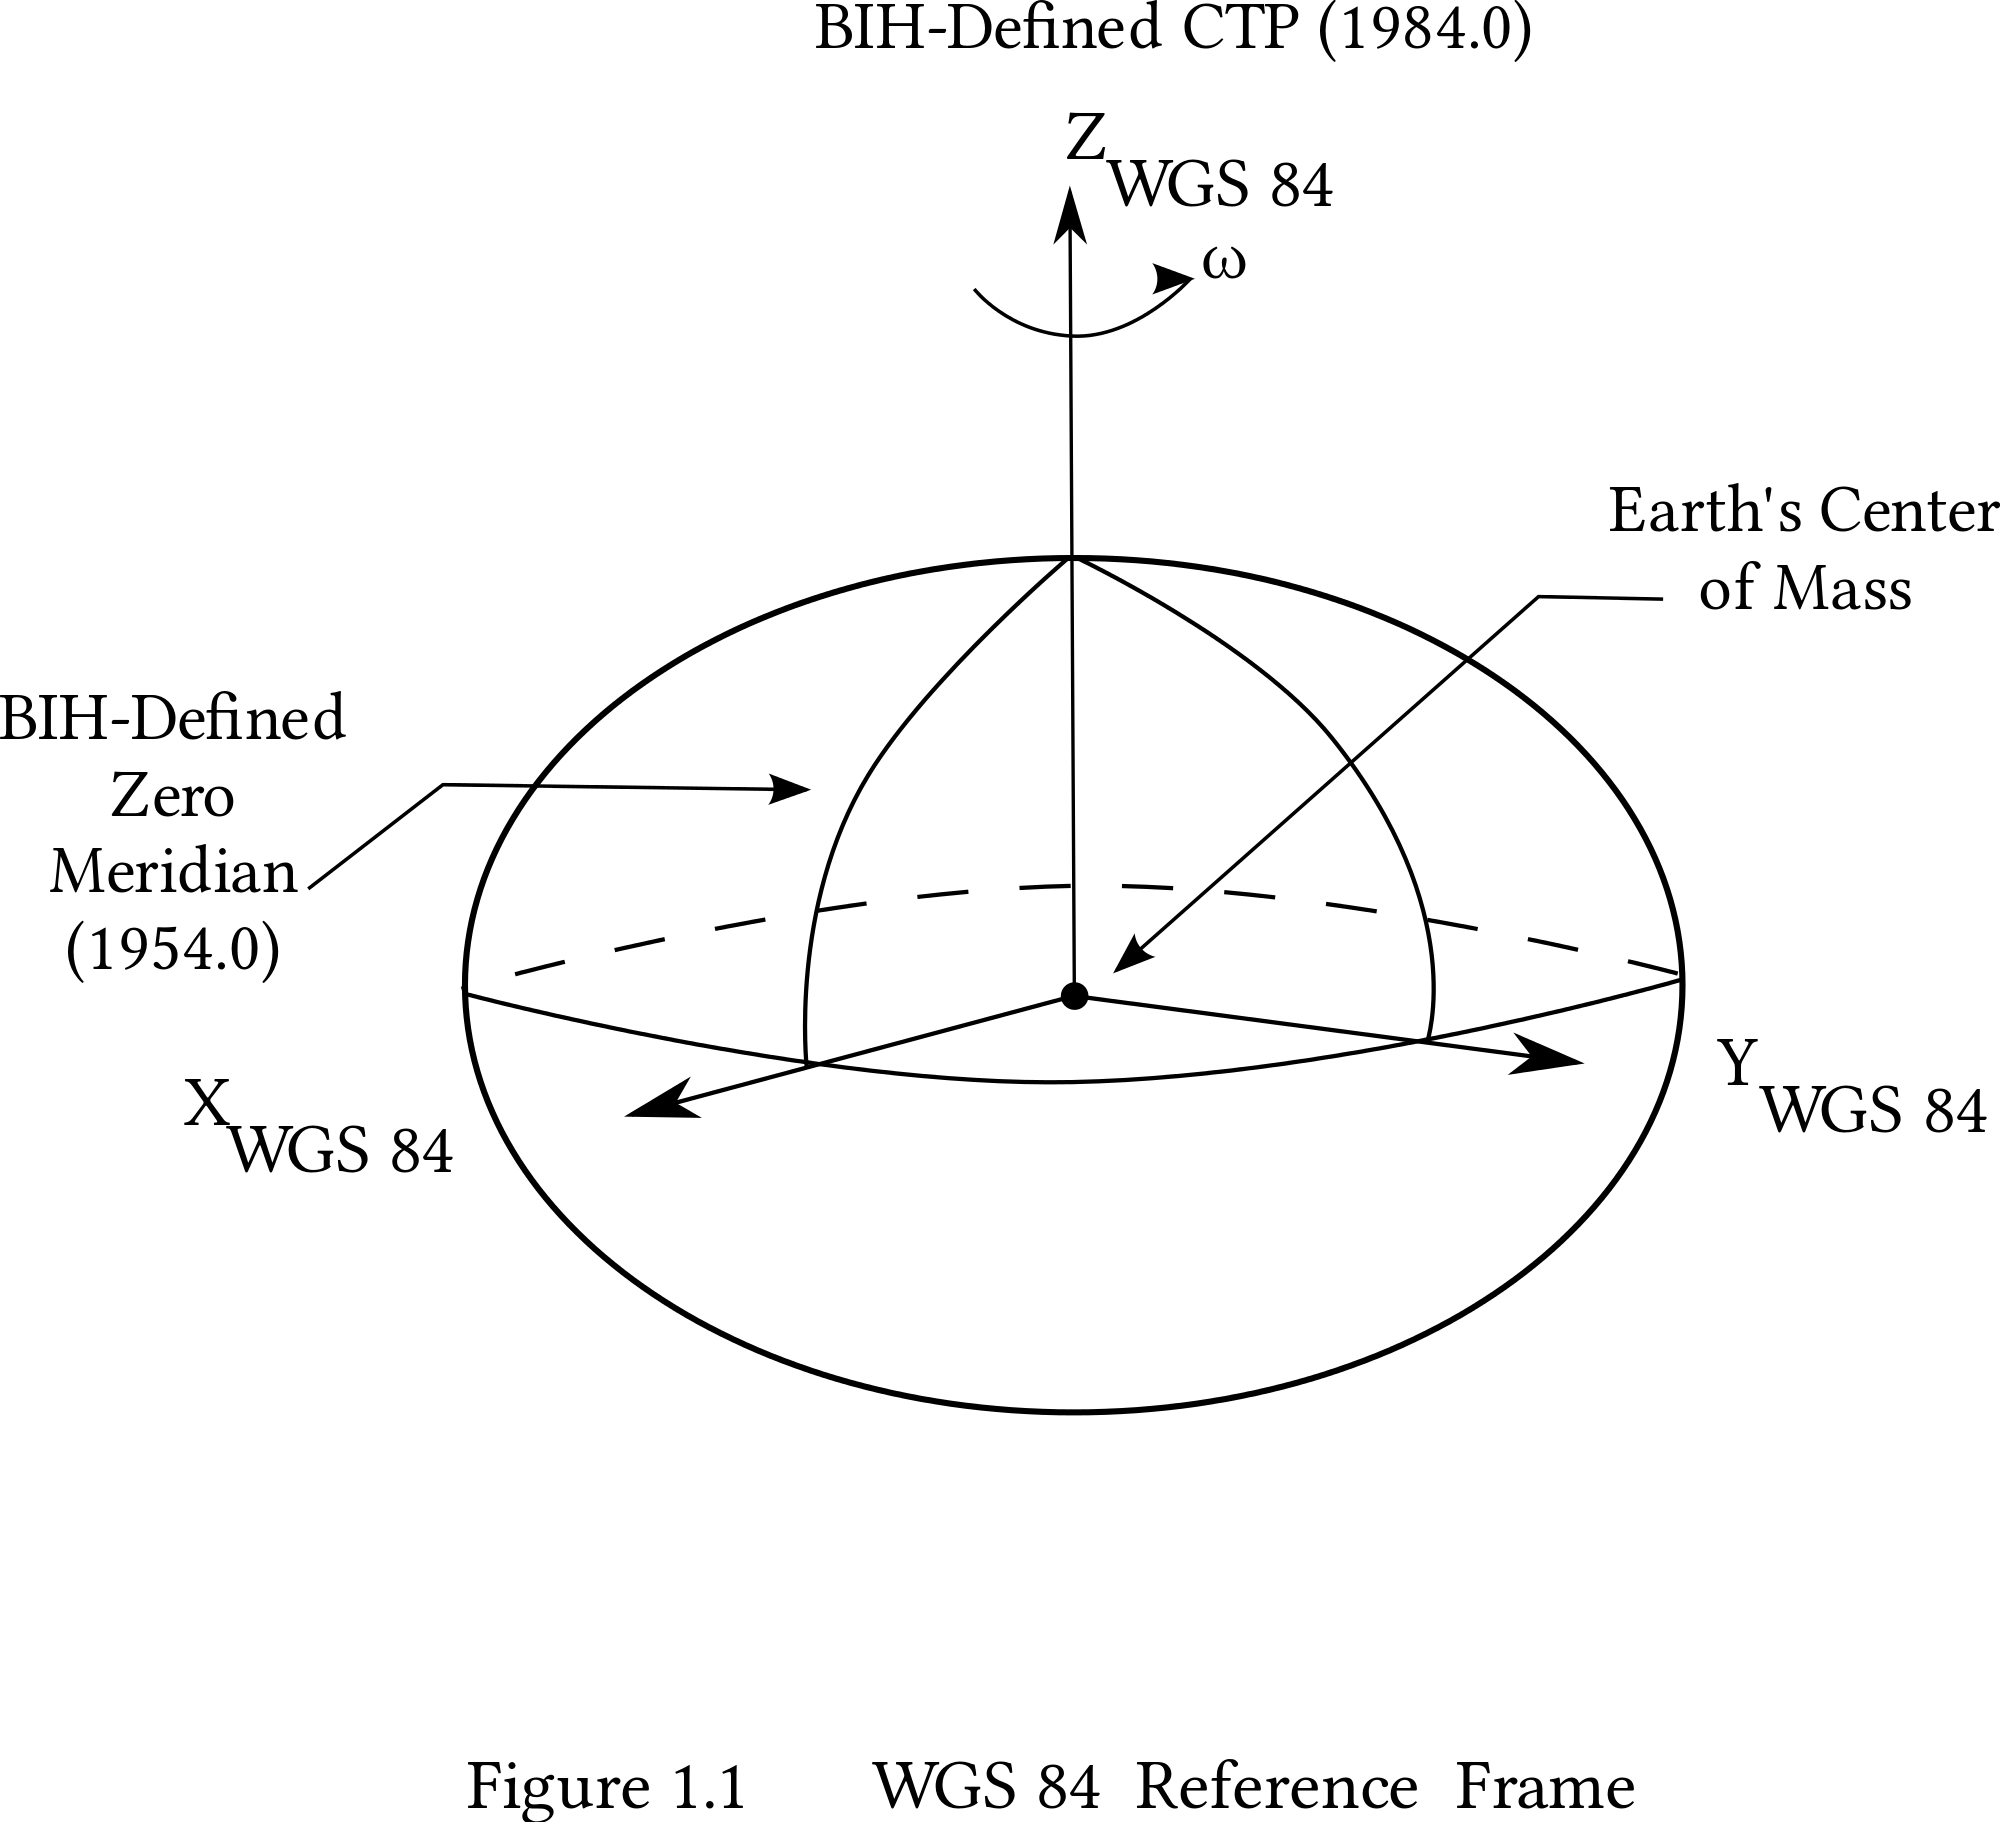
\includegraphics[width=0.3\textwidth, trim={0 9cm 0 3cm},clip]{pix/WGS_84_reference_frame.png}
 % WGS_84_reference_frame.png: 2000x1822 px, 72dpi, 70.56x64.28 cm, bb=0 0 2000 1822
 \caption[Schematische Darstellung des Koordinatensystems WGS84 - Bildquelle: \url{https://commons.wikimedia.org/wiki/File:WGS_84_reference_frame_(vector_graphic).svg}]{Schematische Darstellung des Koordinatensystems WGS84}
 \label{fig:wgs84}
\end{figure}





    
% END

% BEGIN -- Software
    \subsection{Network Common Data Format}
    
    Das Network Common Data Format (NetCDF) dient zum Austausch von wissenschaftlichen Daten. Es ist eine Weiterentwicklung des von der NASA entwickelten Common Data Format (CDF). Das Format zeichnet sich dadurch aus, dass es selbstbeschreibend ist. Dadurch wird die Dokumentation mit den Daten mitgeführt. Dies soll die Portabilität des Datensatzes verbessern.  \footnote{vgl. \cite{FisherNetCDF}}
   
    Neben einigen anderen Sprachen, wurde auch eine Bibliothek für Python entwickelt \footnote{Siehe \cite{netCDF4}} Mit dieser ist es möglich, die Binärdaten zu öffnen und zu numpy-Arrays zu extrahieren. In Listing \ref{lst:example_netcdf} ist die Verwendung exemplarisch an der Extraktion und Berechnung des Datensatzerstellungsdatum aufgezeigt und im Folgenden beschrieben.
    
    \pythonexternal[%
        % ---------------------------------------------
        %   PYTHON netCDF als Beispiel JULD
        caption = {Extraktion und Berechnung des Erstellungsdatums eines NetCDF-Datensatzes},%
        label = {lst:example_netcdf}]%
        {scr/beispiele/netCDF_juld.py}
    
    Um einen Datensatz zu öffnen, bildet man eine Instanz der Klasse \texttt{netCDF4.Dataset}. Die Auswahl des Profils gelingt durch die Pfadangabe als Parameter bei der Instanzierung.
    
    Über das Attribut \texttt{dataset.variables} werden die Datensätze als \texttt{OrderedDict} gehalten. Bei der Extraktion eines Parameters erhält man zunächst die Dokumentation des jeweiligen Datensatzes. In diesem Fall handelt es sich um den Zeitpunkt der Sattelitenübertragung des betreffenden Messprofils.
    
    Aus der Dokumentation lassen sich für die Weiterverarbeitung wichtige Parameter entnehmen.
    So ist der Datensatz in Form des C-Datentyps \texttt{float64} codiert. Beim Datumsformat handelt es sich um \textit{Julian day} ab dem Zeitpunkt \textit{01. Januar 1950}.
    
    Um die Werte eines Datensatzes zu extrahieren, wird über die numpy-slicing Operation \texttt{arr[::]} der Datensatz in vektorieller Form extrahiert. Da in diesem Array nur ein skalarer \texttt{float64} Wert enthalten ist, kann dieser als nulltes Element extrahiert werden.
    
    Zur Überführung in das Format des durch die ISO 8601 bei uns normierten Gregorianischen Kalenders wird ein Datumsobjekt des Referenzdatums benötigt. Durch die Verwendung von \texttt{timedelta} werden die Tage aus dem Feld \texttt{JULD} addiert. Da ein Messzyklus 10 Tage andauert, kann an dieser Stelle der Datensatz durch die Entferndung der Dezimalstellen vereinfacht werden. Die Casting-Operation \texttt{int()} rundet in jedem Fall ab.
    


% BEGIN JULDATE
%END
        

 
   
